\subsection{Definições Preliminares}
Antes de abordarmos (nas próxima seções) alguns aspectos de topologia algébrica, é interessante introduzir as definições de geodésica e quasi-isometria, que serão úteis adiante.

\subsubsection{Geodésicas}
É comum, em muitas aplicações em topologia, uma tentativa de definir e estudar, para espaços gerais, conceitos geométricos intuitivos simples. Nesse contexto, podemos entender as geodésicas como uma tentativa de generalizar, para espaços métricos abstratos, as linhas retas entres dois pontos do plano cartesiano.

Primeiro algumas definições. Seja $(X, d)$ um espaço métrico qualquer. É interessante definir em $X$ o conceito de comprimento para percursos entre pontos.

\begin{definition}
Para um caminho $\alpha$ de $X$ (no sentido topológico, uma função contínua $\alpha : [0,1] \rightarrow X$), definimos o \textbf{comprimento} $l(\alpha)$ conforme
\[
l(\alpha) = \sup_{0=t_0 \leq ... \leq t_n = 1} \sum_{i=0}^{n-1}  d(\alpha(t_i), \alpha(t_{i+1})).
\]
\end{definition}

Para compreender a definição, apelamos à intuição geométrica do plano real. Nesse contexto, dada uma curva $C$ qualquer, podemos aproximar $C$ por um conjunto segmentos de reta (a curva para a qual o comprimento é igual à distância entre as suas extremidades) ligando pontos pertencentes a $C$ e o comprimento da reta é conforme implicado pela definição.

Em suma, entendemos aqui o comprimento de uma curva como o limite superior da soma de distâncias implicadas por qualquer "discretização" desta (no sentido em que, escolhendo mais e mais pontos pertencentes à curva, a soma das distâncias sucessivas entre esses tende ao comprimento em questão).

Da definição, segue imediatamente que, para todo $\alpha$, temos $l(\alpha) \geq d(\alpha(0), \alpha(1))$. Ou seja, todo caminho entre dois pontos tem comprimento maior ou igual que a distância entre suas extremidades (chamamos extremidades de $\alpha$ os pontos $\alpha(0)$ e $\alpha(1)$).

Agora, da intuição de reta, queremos que uma geodésica seja o caminho para o qual o comprimento é igual à distância entre as suas extremidades. Podemos então definir geodésica e espaço geodésico.

\begin{definition}
O caminho $\alpha$ de $X$ é uma \textbf{geodésica} $\iff l(\alpha) = d(\alpha(0), \alpha(1))$.
\end{definition}
\begin{definition}
Caracterizaremos o espaço métrico $X$ como \textbf{espaço geodésico} se e somente se, entre quaisquer dois pontos $x, y \in X$, houver uma geodésica $\alpha$ tal que $x = \alpha(0)$ e $y = \alpha(1)$.
\label{esp_geo}
\end{definition}

Convém abordarmos alguns exemplos de espaços geodésicos e não geodésicos.

Comecemos pelo já citado, observando que $\mathbb{R}^n$ é geodésico. Para verificar basta notar que o segmento de reta entre dois pontos tem comprimento igual à distância entre eles. Ou seja, para quaisquer $a, b \in \mathbb{R}^n$, definimos $r_{a,b}:[0,1] \rightarrow \mathbb{R}^n$ tal que $r_{a,b}(t) = a + t(b-a)$. Note que, da definição, o segmento $r_{a,b}$ é geodésica, pois $l(r_{a,b}) = d(a, b)$ e, como é possível definir geodésica para qualquer par de pontos, o $\mathbb{R}^n$ é de fato geodésico.

Um exemplo de espaço não geodésico pode ser construído a partir do anterior. Tomemos $X = \mathbb{R}^n \setminus {0}$. Note que, para todo $x \in X$, não existe geodésica entre $x$ e $-x$ e portanto $X$ não é geodésico.

Também é interessante notar que, mesmo em um espaço geodésico, as geodésicas entre pontos não são necessariamente únicas. Veja, por exemplo, o próprio $\mathbb{R}^n$ munido da métrica do taxista (induzida pela 1-norma), onde existem infinitas geodésicas entre dois pontos.

\subsubsection{Quasi-isometrias}
Quasi-isometrias são funções que, como qualquer um poderia adivinhar, são "parecidas" com isometrias. Relembremos que isometrias são funções entre espaços métricos que preservam distância entre pontos. Quasi-isometrias, por sua vez, são funções que "nunca distorcem demais" as métricas em questão.

Definamos precisamente. Sejam $(X, d_X)$ e $(Y, d_Y)$ espaços métricos arbitrários e tomemos quaisquer $K, C \in \mathbb{R}_{\geq 0}$.

\begin{definition}
Chamaremos de \textbf{mergulho $\mathbf{(K, C)}$-quasi-isométrico} uma função $f:X \rightarrow Y$ tal que, $\forall x, y \in X$,
\[
\frac{d_X(x, y)}{K} - C \leq d_Y(f(x), f(y)) \leq K d_X(x, y) + C.
\]
\end{definition}
\begin{definition}
Chamaremos de \textbf{$\mathbf{C}$-grossamente sobrejetiva} uma função $f:X \rightarrow Y$ para a qual, $\forall y \in Y \ \exists x \in X$ tal que $d_Y(f(x), y) \leq C$.
\end{definition}
\begin{definition}
Chamaremos de \textbf{$\mathbf{(K, C)}$-quasi-isometria} um mergulho (K, C)-quasi-isométrico que é C-grossamente sobrejetivo.
\end{definition}

Visualizemos um exemplo de quasi-isometria (omitiremos a partir daqui os parâmetros $K$ e $C$ respectivos quando for trivial sua descoberta).

Observe a figura \ref{figure:cay(Z)}. Assuma que cada um dos elementos conexos sejam espaços métricos em que as arestas tem todas comprimento unitário e que encontram-se apenas nos nós. Além disso, assuma que ambos os espaços sigam indefinidamente com o padrão geométrico para a direita e esquerda.

Tomemos a função $f$ de projeção (ou seja, a função que, para todo ponto do espaço acima assinale o ponto o ponto do espaço abaixo que "encontra-se na mesma vertical") do primeiro, chamemos $X$, no segundo, chamemos $Y$.

Note que a função de projeção é $(3,0)$-quasi-isometria, pois, dados $x, y \in X$, a distância entre dois pontos $f(x)$ e $f(y)$ nunca é mais de três vezes maior ou menor que entre $x$ e $y$.

Também é interessante perceber a implicação de que toda função $g: Y \rightarrow X$ tal que $\forall y \in Y$ temos $y = f(g(y))$ também é quasi-isometria.

Enfim, a visualização dos espaços da figura \ref{figure:cay(Z)} permite solidificar a intuição de que "são quasi-isométricos os espaços que, de longe, parecem iguais".

\begin{figure}[ht]
  \centering
  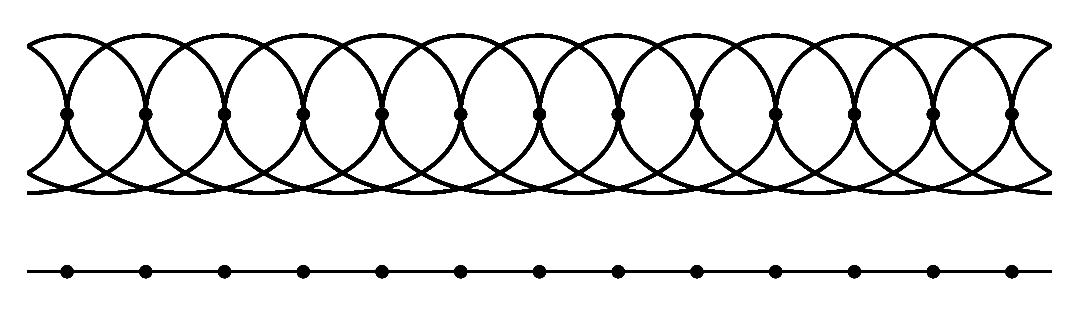
\begin{tikzpicture}
    \begin{scope}
    \clip (-6.5,-0.2) rectangle (6.5,3.1);

    \foreach \x in {-6,-5,...,6}{% Two indices running over each
      \foreach \y in {-6,-5,...,6}{% node on the grid we have drawn 
        \draw[line width=1pt](\x-1,0)--(\x+1,0);
        \node[draw,circle,inner sep=1.5pt,fill] at (\x,0) {};
            % Places a dot at those points
      }
    }
    
    \foreach \x in {-6,-5,...,6}{% Two indices running over each
      \foreach \y in {-6,-5,...,6}{% node on the grid we have drawn 
        \node[draw,circle,inner sep=1.5pt,fill] at (\x,2) {};
        \draw[very thick] (\x,2) arc[start angle=0, end angle=180, x radius= 1, y radius = 1];
        \draw[very thick] (\x+2,2) arc[start angle=0, end angle=180, x radius= 1, y radius = 1];
            
        \draw[very thick] (\x,2) arc[start angle=0, end angle=-180, x radius= 1.5, y radius = 1];
        \draw[very thick] (\x+3,2) arc[start angle=0, end angle=-180, x radius= 1.5, y radius = 1];
      }
    }
    \end{scope} 
  \end{tikzpicture}
  \caption{Dois espaços dentre os quais é possível traçar uma quasi-isometria.}
  \label{figure:cay(Z)}
\end{figure}